\chapter{Thermal Design and Building Envelope}

The building function which has been chosen for study as the optimisation objective function is the thermal function of building envelopes. This chapter breaks down the subject into the basic scientific concepts behind the thermal perforamce of the building envelope and how it is perceived by the users or occupants of internal building spaces. 

\paragraph{The Science of Thermal Design}\mbox{}\\

The basis on which thermal design is built is mainly that of simple physics, and physiology. The physics is the science that describes the building, it's components and it reactions to it's external environment, sometimes also includes other elements of the equation of thermal design such as clothing or furniture. As for the physiological part, it's concern is the occupant; the human being. It describes the way our bodies react to our environment, which is in this case the micro-climate created by the building.

The elements of thermal design are the occupant, the building and the environment. An integral part of this chapter is also dedicated to the definition of what is called the building 'envelope', it's thermal behaviour and the projection of thermal design principles on this prominent part of buildings.

\paragraph{Sustainability Aspects of Thermal Design}\mbox{}\\

An important question that may come to mind is how thermal design is concerned with green or sustainable architecture. Consider the following: in some countries such as the UK, buildings have a 50\% share of the countries energy consumption, of which 60\% is used only by houses, and half of which is used in space heating alone \cite{edwards96}. In other countries with hotter climates such as Abu Dhabi, cooling energy consumption had risen from 1625 MW to 4750 MW of power from 1990 to 2007 \cite{nauman07}. Many other examples similar to the above would lead to the conclusion; that heating and cooling of spaces are major consumers of energy, demanding more fuel combustion as a means of electricity generation in most cases, which in turn increases CO\textsubscript{2} emissions. So if we were to state how thermal design is vital for sustainable building design, we could say that it allows for CO\textsubscript{2} emission reduction, a better management of resources and a thermally comfortable space for different activities.

\label{BuildEnvDef}
\subsection{The Building Envelope}
A building envelope is the components which separate the indoor spaces from the outdoors. These components include all `physical' barriers such as walls, roofs, windows, doors and foundations \cite{HPO}. The main functions of a building envelope -or `enclosure'- are \cite{straube05}:
\begin{enumerate}
  \item Structural support and load-bearing.
  \item Control of inward and outward flow of energy and matter.
  \item Aesthetic element of interior and exterior.
\end{enumerate}
The only function of concern from the abovementioned in this thesis will be the control of thermal energy, which will narrow our scope throughout this chapter and it's successors.

\section{Physics of Thermal Design}

\subsection{Heat and Temperature}
\paragraph{Heat,}is a form of energy while \textbf{Temperature} is it's symptom. Temperature has a measurement scale of Celsius which is based on water's freezing and boiling points at 0 and 100 degrees, while the Kelvin is used for measuring temperature intervals. \textbf{Specific Heat} provides the connection between heat and temperature. It is equal to the amount of energy; or heat, required to raise the temperature of a unit mass of a substance by 1 degree, measured in J/Kg.K. This attribute is indeed of utmost importance in terms of thermal design, as it defines how different substances respond to heat. Some materials will reach specific temperatures much faster than others and therefore in turn heat surrounding mediums faster. \textbf{Latent Heat} is the amount of heat lost or absorbed when changing form one physical state to another.

\paragraph{Thermodynamics.}Thermodynamics deal with heat flow. The \textbf{First Law} of thermodynamics states that energy cannot be created nor destroyed, but converted from one form to another. The \textbf{Second Law} states that heat can flow in only one direction: from a high temperature point to a low one. The magnitude of such a flow can be measured in two ways:
\begin{inparaenum}
  \item \emph{Heat flow rate}; the total flow in unit time through a defined area which is measured in Watt (W), or
  \item \emph{Heat flux density}; the rate of flow of heat through a unit area, measured in W/m\textsuperscript{2}.
\end{inparaenum}

\subsubsection{Heat Flow}
As stated in the second law of thermodynamics; heat flows from a high temperature point to a low temperature point. This flow occurs in 3 distinct forms:
\begin{enumerate}\label{HeatExchange}
  \item \emph{Conduction}, which occurs within the same medium or through direct contact.
  \item \emph{Convection}, which occurs between different physical forms; such as gas and liquid, or through different mediums; such as liquid transporting heat from one body to another.
  \item \emph{Radiation}, which occurs from a body with warmer \emph{surface} to another which is cooler.
 
\end{enumerate}

The physics that governs these principles of heat transfer has much more detail to it; equations that define the process and it's output and other factors that might affect the physical behaviour of different materials regarding conduction, convection or radiation such as inevitable damage on site that reduces their efficiency. Since we intend to handle matters of calculation regarding thermal design by means of energy simulation applications, only the minimal amount of equations and derivations will be mentioned later in the chapter when needed.

\subsubsection{Psychrometry}
This section will briefly describe the heat flow process when a new element is introduced to the equation; \emph{humidity}. Our purpose is not to illustrate the means of calculation of different processes of heat flow -as with the previous section- which is done through what is called the \emph{Psychrometric Chart}. Our purpose is to demonstrate the general concepts of the process.
\paragraph{Air and Humidity.} Air is composed of a mixture of different gases, Oxygen ($O_2$) and Nitrogen ($N_2$) being the prominent elements. Another element of great importance to our subject is water ($H_2O$). It plays a key role in thermal comfort. Water is carried by the air in it's gaseous state; water vapour. Air can carry a limited amount of water, this amount changes according to air temperature, whenever this limit is reached, the air is said to be \emph{Saturated}. The amount of water vapour -or \emph{Humidity} as we shall refer to it henceforward-, is measurable on two scales; \emph{Absolute} and \emph{Relative} humidity. Absolute Humidity measures the weight of water vapour in grams for each Kilogram of air (g/Kg), while relative humidity measures the percentage of maximum amount of water vapour supported by air at a given temperature; or \emph{Saturation Humidity}.

\paragraph{Enthalpy.}It is the heat content of air, relative to the heat content 1 Kg of air at $0^\circ$ Celsius and 0 humidity. We can derive two different components of air heat content; 
\begin{inparaenum}
\item \emph{Sensible Heat}; the amount of heat raising dry bulb temperature, and
\item \emph{Latent Heat}; the amount of heat evaporating water to it's gaseous state and forming air humidity.
\end{inparaenum}

\paragraph{The Psychrometric Chart.}As mentioned earlier; the psychrometric chart (figure \ref{PsychroChart}) is used to calculate different exchanges of heat and humidity, these exchanges are called \emph{Psychrometric processes}. The processes can be summarised to:
\begin{enumerate}
  \item \emph{Heating} and \emph{Cooling}, at which the our point of reference on the chart moves right and left, respectively, are the processes of raising and lowering of dry-bulb temperature, respectively.
  \item \emph{Humidification}, is the evaporation of water by heat into the air reducing dry-bulb temperature and increasing humidity\footnote{The word \emph{Adiabatic Humidification} is sometimes used to designate that no sensible heat is introduced in the process.}. The point of reference moves diagonally up to the left on the chart as an indication of this process.
  \item \emph{Adiabatic Dehumidification}, is the removal of humidity by means of passing the air through a chemical sorbent\footnote{\emph{Sorb}: to take up and hold by either adsorption or absorption \cite{merriam03}}, which removes some of the moisture content, releasing heat and increasing dry-bulb temperature while reducing humidity.
\end{enumerate}

\begin{sidewaysfigure}[htbp] %[Here Top Bottom nextPage]
\centering
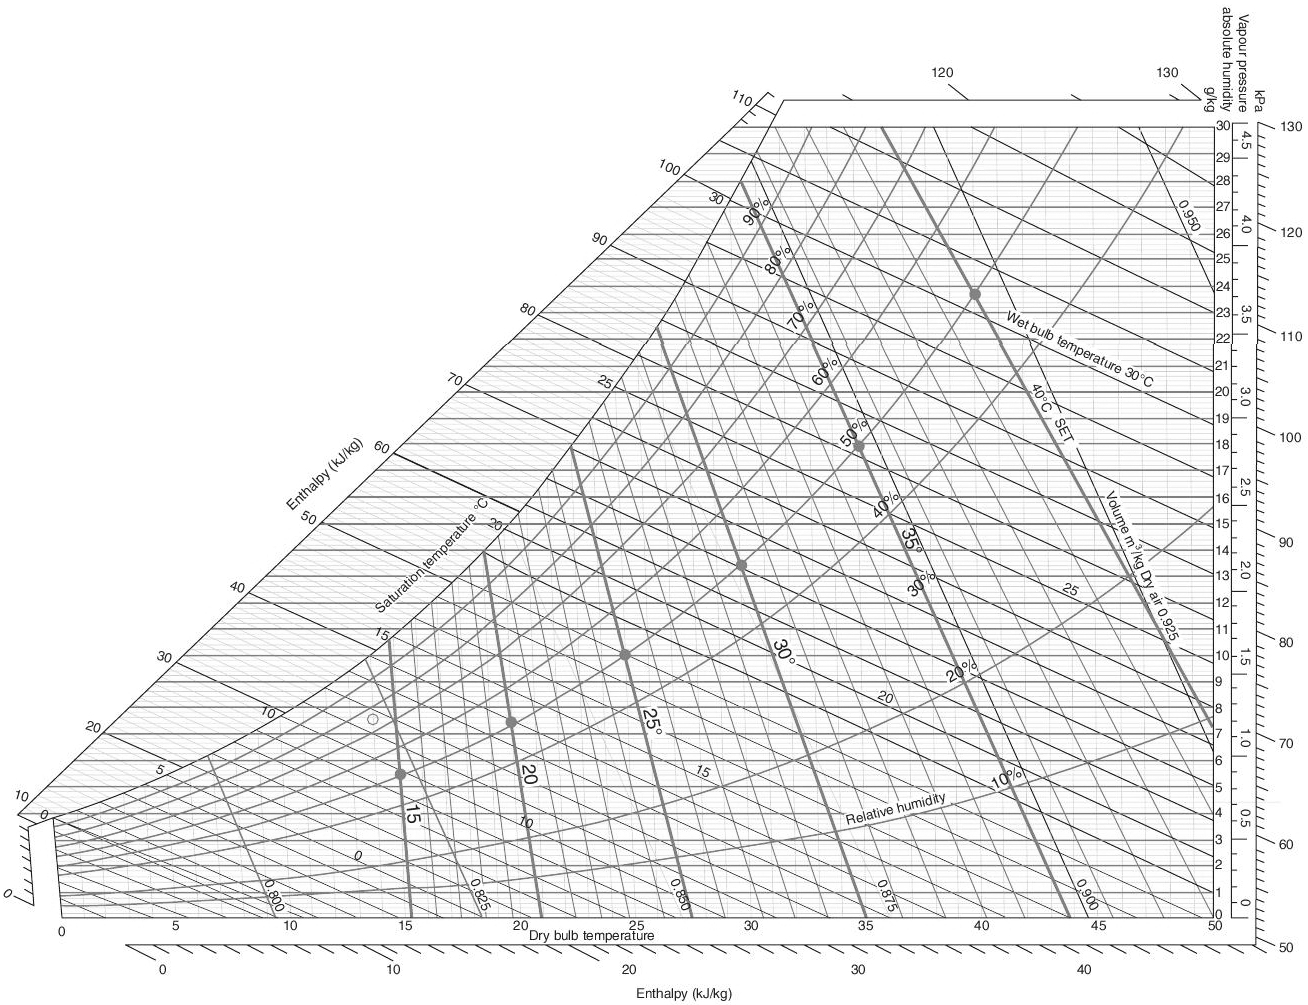
\includegraphics[width=0.9\textwidth]{./Images/1-PsychrometricChart}
\caption[The Psychrometric Chart]{The Psychrometric Chart \cite{szokolay08} \label{PsychroChart}}
\end{sidewaysfigure}

\newpage
\section{Thermal Comfort}
\label{sec:ThermalComfort}

Thermal design in principle is controlling indoor temperature, to increase or decrease gained heat.  If we were to say that our main concern is energy efficiency and sustainability, one might think that this kind of endeavour does not concern the occupant; a simple matter of saving electricity through energy efficiency. Such an assumption would be completely ignoring the fact that it is the occupant's feeling of discomfort that triggers the need to heat or cool a space using air conditioning; thus using more power.
\subsection{Equilibrium and The Factors of Thermal Comfort}
Thermal comfort is simply a matter of balance; the balance of gained and lost heat by the human body such as metabolism and different heat exchange methods (section \ref{HeatExchange}). An equation can be formulated to illustrate this exchange as:
\begin{equation}
M \pm Rd \pm Cv \pm Cd - Ev = \Delta S
\label{StoredHeat}
\end{equation}

\begin{minipage}{\dimexpr\textwidth-3cm}
{\footnotesize Where: $M=$ Metabolic rate, $Rd=$ net radiation exchange, $Cv=$
convection, $Cd=$ conduction, $Ev=$ evaporation and $\Delta S=$ change in stored heat.}
\end{minipage}\\\\\\
The factors of this equation of balance; or thermal comfort are described by S.  Szokolay \cite{szokolay08} as being of three main types or categories. These types are environmental, personal and contributing factors.
\newline

\begin{table}[htbp]
\centering
\begin{tabular}{lll}
\hline
Environmental	& Personal			& Contributing Factors\\ \hline
Air Temperature	& Metabolic Rate	& Food and Drink\\
Air Movement	& Clothing			& Body Shape\\
Humidity		& State of Health	& Subcutaneous Fat\\
Radiation		& Acclimatisation	& Age and Gender\\
\hline
\end{tabular}
\caption[Factors of Thermal Comfort]{Factors of Thermal Comfort \cite{szokolay08}}
\label{FactorsOfComfort}
\end{table}

\subsection{Homoeothermy}
\paragraph{Homoeothermy,}is the ability of a body to adjust it's internal temperature through different means such as sweating to reduce body heat by evaporation, or shivering to induce heat.  Basic methods though are not that prominent, which are \emph{vasoconstriction} and \emph{vasodilation}; the reduction and increase of blood flow to the skin, respectively, to conserve body heat in cold climates and to release it in warmer climates. These are important factors to be considered, so as to not treat the body as a passive thermostat, and compensate for such reactions when designing a thermal space. There are other physiological changes in reaction to cold and warm weather that occur on the long term such as change in metabolism rate that we will not delve into.

\paragraph{Psychological perception,}is another aspect of how we conceive temperature. This is mainly a matter of expectation. Any given temperature will be perceived differently according to prevailing temperatures of a particular month or season, so if we were to say that outdoor temperature and wind speed are $24^\circ C$ and $0.2 m/sec$, it might be perceived as mildly cold in a summer season, or mildly warm in an autumn season. The following figure (\ref{PsychoPhysioModel}) illustrates the psycho-physiological model of thermal perception \cite{szokolay08}.

\begin{figure}[htbp]
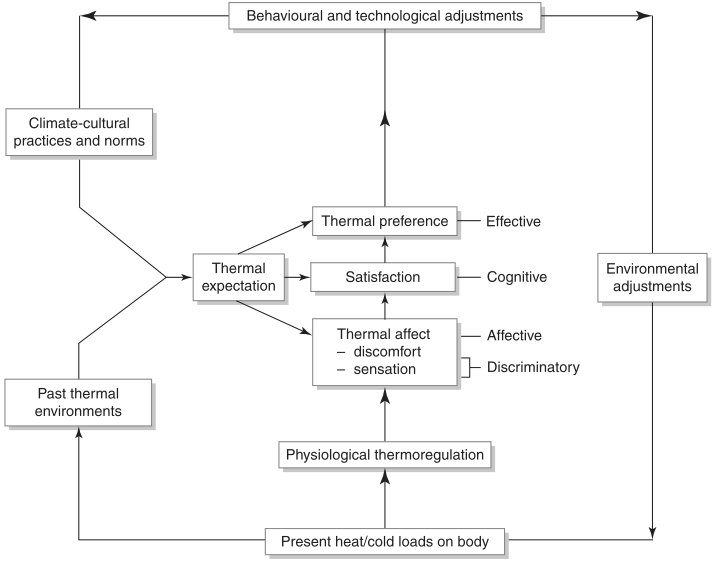
\includegraphics[width=13.5cm]{./Images/2-PsychoPhysioModel}
\caption[Psycho-Physiological Thermal Perception Model]{Psycho-Physiological Thermal Perception Model \cite{szokolay08} \label{PsychoPhysioModel}}
\end{figure}

\subsection{Comfort Indices}
Since thermal comfort is affected by multiple environmental aspects, a unified index was needed to define environmentally accepted conditions. Many indices have proposed and accepted over the years including the famous chart made by Victor Olgay. One index which has been introduced lately and is widely accepted is the ET* (ET star), or it's standardised version the \textbf{SET}. The SET index is superimposed upon the Psychrometric chart (Fig. \ref{PsychroChart}) coinciding with DBT at 50\% RH curve until it reaches $14^\circ C$, then slanting gradually, demonstrating that higher humidity lowers the tolerance for temperature of occupants.

\section{Climate}
This section deals with the element of thermal design which defines the external environmental factor; climate. Although it is a complex system with many aspects (radiation, wind speed, wind temperature, precipitation\ldots etc.), we shall discuss exclusively the environmental aspect of the Sun. This choice has been made in order to simplify experimentation with algorithmic design of building envelope through our focus on one element of the heat exchange process.

\subsection{The Sun}
Szokolay \cite{szokolay08} argues that the aspects essential for a designer to understand are the movement of the Sun\footnote{This is a reference to it's apparent movement as a result of the actual movement of Earth in it's orbit.}, and how to utilise or diminish it's effect.\\ The Earth's orbit around the sun has unique characteristics such as it's slanted rotational axis relative to it's orbital axis around the sun, creating difference in temperatures across the year; creating seasons. This phenomenon also results in the difference in day and night lengths depending on the distance from the Earth's equinox\footnote{The point at which the Earth's equator is on the same plane with the Sun's centre.}. These characteristics are discussed in detail in many publication, but our main concern is the resulting movement of the sun.

\subsubsection{Sun-path Diagrams}
The essential tool of studying the Sun's movement is the Sun-path diagram. This diagram displays the Sun's position at any given date, time and global position. The position of the Sun is marked all year round on projection of the sky represented as a dome or hemisphere, with the the desired position on land being it's centre, this view is called a \emph{Lococentric} view (Figure \ref{Lococentric}) The most common projection is called the \emph{Stereographic} projection (Figure \ref{Stereographic}).

\begin{figure}[htbp]
\centering
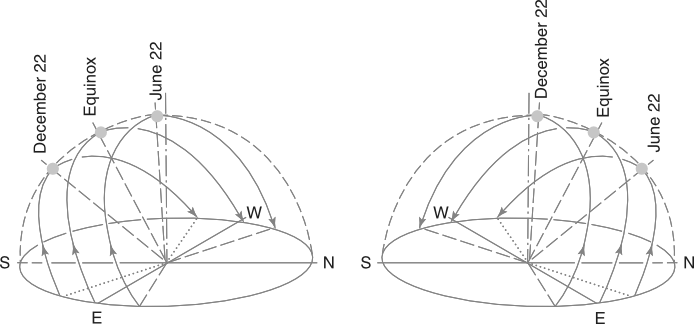
\includegraphics[width=10cm]{./Images/3-Lococentric}
\caption[Lococentric Sun Path View]{Lococentric View \cite{szokolay08}}
\label{Lococentric}
\end{figure}

\begin{figure}[htbp]
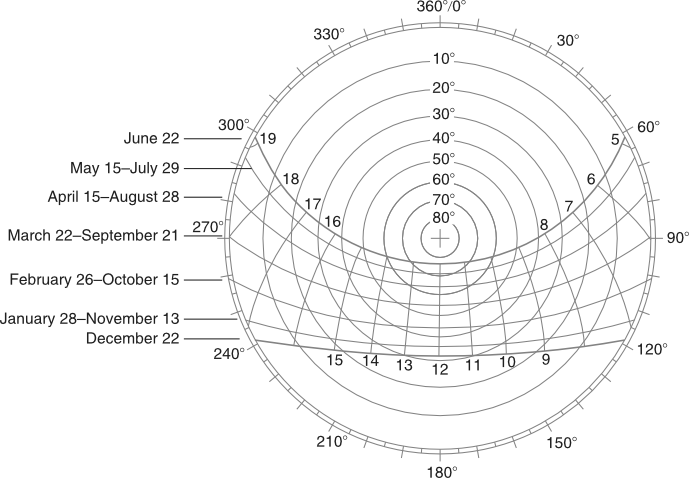
\includegraphics[width=\textwidth]{./Images/4-Stereographic}
\caption[Stereographic Sun-Path Projection] {Stereographic Sun-Path Projection \cite{szokolay08}}
\label{Stereographic}
\end{figure}

\subsubsection{Solar Radiation}
Perceivable solar radiation by humans is partitioned into three ranges:
\begin{enumerate}
  \item UV radiation, which is of $20-380nm$ wave-length.
  \item Visible light, ranging in a spectrum of violet to red, $380-700nm$ length.
  \item Short infra-red\footnote{Also described as \emph{thermal radiation}}, ranging from
  $700-2300nm$.
\end{enumerate}
The amount of irradiation\footnote{Energy flow density integrated over a period of time, measured in $Wh/m^2$} differs from one location to the other. There are causes of this phenomenon\cite{szokolay08}, which are:
\begin{enumerate}
  \item Angle of incidence, changing according to the angle of the earth's axis relative to it's solar orbit.
  \item Atmospheric depletion, depending on altitude; the distance which the radiation has to travel.
  \item Duration of sunshine, depending on day length and local topography.
\end{enumerate}

\section{Thermal Behaviour of Buildings}
\label{sec:ThermalBehaviour}
Buildings have a thermal system very similar in concept to thermal comfort (equation \ref{StoredHeat}), it is an equation of heat gain and loss, but with the minor difference that thermal comfort is essentially defined by equilibrium, while thermal behaviour of buildings is not.\\ The defining equation of thermal behaviour of buildings is as follows:
\begin{equation}
Qi \pm Qc + Qs \pm Qv - Qe = \Delta S
\end{equation}

\begin{minipage}{\dimexpr\textwidth-3cm}
{\footnotesize Where: $Qi=$ internal heat gain, $Qc=$ conduction heat gain or loss, $Qs=$ solar heat gain, $Qv=$ ventilation heat gain or loss, $Qe=$ evaporation heat loss and $\Delta S=$ change in stored heat.} \end{minipage}\\\\\
An important fact is that solar radiation is the most significant energy input in the equation\cite{szokolay08}, this is reassuring since we have chosen to take the solar element into account exclusively throughout the entire dissertation as mentioned earlier.

\subsection{Solar Control}
The idea behind algorithmic design -in our particular case- is controlling the design process in order to produce a favourable condition. Since we have narrowed our scope to the issue of solar design, our favourable condition will depend on the introduction or prevention of solar radiation.  The unfavourable solar radiation period causing overheating is marked on the sun path diagram, showing the angles at which the sun casts it's unwanted rays, then superimposed on a diagram with the opening's orientation on which our shading instrument is designed creating a shading mask.

\subsubsection{Shading Design}
\label{Shading}
Shading is the proven most efficient way of controlling solar radiation externally. External shading is divided into to categories:
\begin{enumerate}
  \item	\textbf{Vertical Shading}, this type is characterised by by horizontal shadow angles (HSA), examples of which are vertical louvres (fig. \ref{HSA}).
\begin{figure}[htbp]
\centering
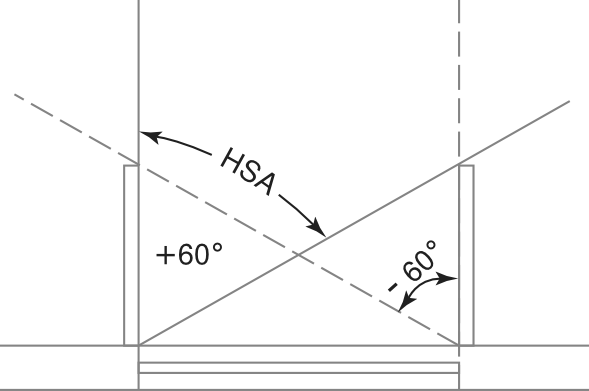
\includegraphics[width=5cm]{./Images/5-HSA}
\caption[Horizontal Shadow Angle]{Horizontal Shadow Angle \cite{szokolay08}}
\label{HSA}
\end{figure}
  \item \textbf{Horizontal Shading}, are characterised by vertical shadow angles (VSA), examples of which are horizontal louvres and canopies (fig. \ref{VSA}).
\begin{figure}[htbp]
\centering
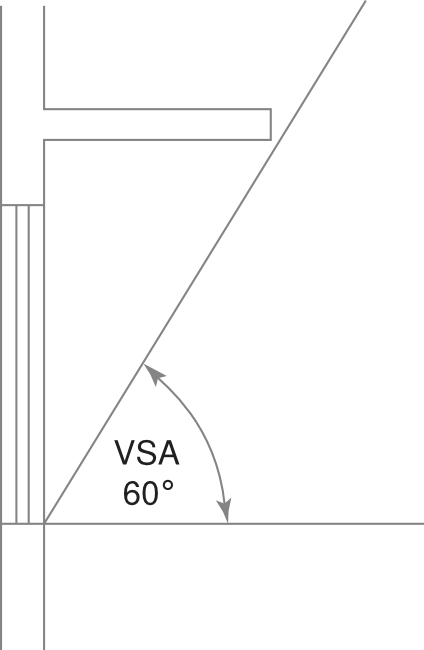
\includegraphics[width=3cm]{./Images/6-VSA}
\caption[Vertical Shadow Angle]{Vertical Shadow Angle \cite{szokolay08}}
\label{VSA}
\end{figure}
  \item \textbf{Solar VSA}, identical to VSA unless not on the vertical plane of the surface normal of the building (fig. \ref{EggCrate}).
  \item \textbf{Egg-crate Shading}, complex shading devices combining all previous shading masks.
\begin{figure}[htbp]
\centering
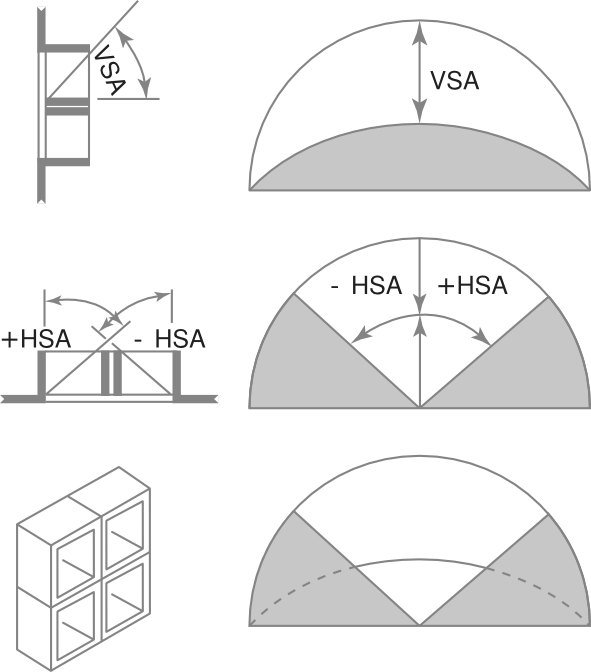
\includegraphics[width=6cm]{./Images/7-Egg-Crate}
\caption[Egg-Crate Shading Devices]{Egg-Crate Shading Devices \cite{szokolay08}}
\label{EggCrate}
\end{figure}
\end{enumerate}

\subsubsection{Solar Heat Gain}
\label{sec:SolarHeatGain}

Solar heat gain is a product solar radiation, which is divided into 
\begin{inparaenum}
	\item direct beams, 
	\item diffused beams and 
	\item occasional reflected beams.
\end{inparaenum}
Solar heat gain is calculated differently depending on whether it is opaque or transparent.

\paragraph{Transparent elements,}such as glazing, receive solar radiation and produce and amount of solar heat gain depending on it's surface area ($A$) and the materials solar gain factor ($\theta$). The incident rays are divided into transmitted rays($\tau$), reflected rays ($\rho$) and absorbed rays ($\alpha$).
\begin{equation}
\tau + \rho + \alpha = 1
\end{equation}
The absorbed portion of solar rays is then emitted to the outside and the inside through convection and radiation, adding to the amount of heat transmitted through the glass to the inner space, thus producing solar heat gain.
\begin{equation}
Qs=A\times G\times \theta \label{TransHeatGain}
\end{equation}

\paragraph{Opaque elements}are treated differently. The input radiant heat depends on the surface absorptance ($\alpha$): 
\begin{equation}
Q_{in}=G\times A\times \alpha
\label{OpInRad}
\end{equation}
The heat input will raise surface temperature ($T_s$), causing heat loss to the air, which depends on surface conductance ($h$): $Q_{loss}=A\times h\times (T_s\times T_o)$, $T_o$ being air temperature.\\
When the surface reaches equilibrium; i.e. $Q_{in}=Q_{loss}$, or:
\begin{equation}
G\times A\times \alpha = A\times h\times (T_s\times T_o)
\end{equation}
We can derive $T_s$ as:
\begin{equation}
T_s=T_o+G\times \frac{\alpha}{h}
\end{equation}
Bear in mind that this value is of a ``sol-air'' temperature; which neglects the transfer of heat from the surface into the body of the element \cite{szokolay08}. Thus, we deduce that the heat flowing through an opaque element can be calculated as:
\begin{equation}
Q_c=A\times U \times (T_s-T_i)
\newline
\end{equation}
\center{ \footnotesize Where $U$ is the air to air thermal transmittance, \\and $T_i$ is the internal air temperature}
\flushleft

\subsection{Steady State Heat Flow}
\paragraph{Conduction heat flow,}(see section \ref{HeatExchange}) is calculated as the product of $A\times U\times \Delta T$. In our case we will use the accumulated area and transmittance of the building envelope; referred to as \emph{envelope conductance}.
\begin{equation}
Q_c=\sum(A\times U)\times \Delta T
\label{EnvConduct}
\end{equation}
{\footnotesize Where $\Delta T$ is equal to the difference between outdoor and indoor temperatures $T_o-T_i$}

\paragraph{Thermal bridges,}
All heat flow calculations hitherto are true only when heat flow is ``one-dimensional'' \cite{szokolay08}; assuming that incident radiation is in the surface normal direction, and that the envelope element is quite large, flat, solid and of uniform construction material and geometry---which is rarely the case, if ever.\\
This shows that heat flow calculations are an approximation. Here the concept of thermal bridges should be introduced, which cause heat to flow in two or three dimensions, caused by geometrical variation or construction material differences in one building element (figure
\ref{ThermalBridges}).
\begin{figure}[htbp]
\centering
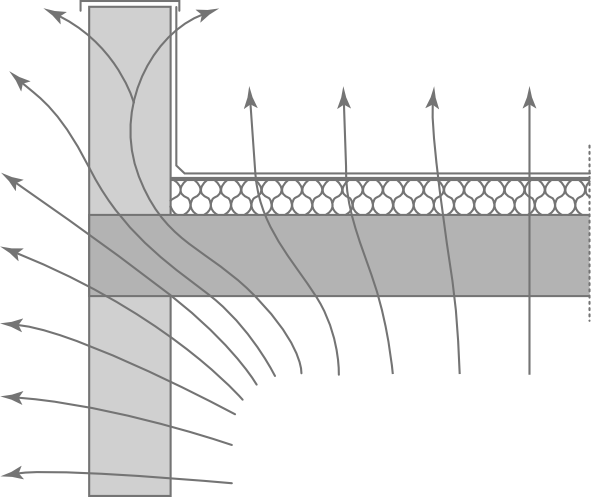
\includegraphics[width=6cm]{./Images/8-ThermalBridges}
\caption[Thermal Bridges]{Thermal bridges caused by geometrical and material variation
\cite{szokolay08}} \label{ThermalBridges}
\end{figure}


\label{sec:ThermalDesignVariables}
\section{Thermal Design Variables}
\label{sec:ThermalDesignVariables}

An integral part, and arguably the most important one of this chapter, is where we demonstrate the different design variables affecting the building thermal performance, or it's envelope. This importance comes from the fact that these variables will be the basis on which we will choose our form generation parameters later on.\\ The most influential traits of any given building as argued by Szokolay \cite{szokolay08} are shape, fabric, fenestration and ventilation. We will demonstrate different attributes with the exception of ventilation.\\ \vspace{0.5cm} \label{ThermDesVar}
\begin{enumerate}
  \item \textbf{Shape}
  	\begin{enumerate}
    	\item \emph{Surface-to-volume ratio}\\ As illustrated before (eqn. \ref{EnvConduct}), heat gain is partially a product of surface area, therefore it is essential to decrease or increase the surface area of a building in relation with it's volume, or to be practical; it's footprint.  For example; if we were to decrease the surface area, the optimum shape would be a spherical/hemispherical one. 
    	\item \emph{Orientation}\\ In order to utilise heat gain and heat dissipation properly, one
    	must consider building shape ration and orientation. Usually elongated northern and southern
    	fa\c{c}ades with a ratio of 2 to 1.3 are suitable for most cases \cite{szokolay08}.
  	\end{enumerate}
  \item \textbf{Fabric}\footnote{Resistive, reflective and capacitive insulation have been omitted from this list, due to it's irrelevance to our scope}
  	\begin{enumerate}
    	\item \emph{Shading}\\ \emph{See section \ref{Shading}}
    	\item \emph{Surface material properties}\\ This is a matter of absorptance and reflectance (refer eqn.\ref{OpInRad}). Generally speaking; a bright colour is reflective, while a dark one absorbs more energy; or heat.
  \end{enumerate}
  \item \textbf{Fenestration}
  	\begin{enumerate}
  	  \item \emph{Size, position and orientation}\\ A fundamental aspect of fenestration and radiation input control\footnote{Also an essential variable of ventilation control}.
  	  \item \emph{Glazing material}\\ Single glazing, double glazing\ldots in addition to glass quality and different unique traits the control heat input.
  	  \item \emph{Closing mechanism}\\ Solutions include fixed glass, louvres and opening sashes.
  	  \item \emph{External Shading}\\ In relation with windows or envelope voids.
  	\end{enumerate}
\end{enumerate}

\clearpage
\section{Simulation}

Simulation is a modelling process which can predict the physical reactions or behaviour of a system. This modelling process would typically use abstract definitions of the system, regardless of many architectural features. The behaviour of the system is described using mathematical formulas, as those provided in this chapter. \cite{fasoulaki08}

\paragraph{Simulation variables and constants.} Throughout the thesis, the notion of variables has been a recurring theme; it has been a key aspect of parametric models, a control element of algorithms and finally a control element of thermal design (\autoref{ThermDesVar}). In simulated environments; the mathematical formulas introduce constants and variables necessary for governing the system. The power of simulation techniques and software come from the fact that by modifying the system variables; the designer can \emph{measure the impact of variable value modification on the system's performance}. However, a disadvantage of simulation is that in order to reach an optimum, or even acceptable results, the designer must work under a process of trial and error. The designer would then examine the feedback given by the simulation process, modify the variable values accordingly and reiterate the process in a very inefficient manner. \cite{fasoulaki08}

\paragraph{Simulation, Algorithm and Thermal Design.} When the designer finds himself at a disadvantage due to the impractical process of trial and error; \emph{the importance of automation of the design process through algorithmic design becomes evident}. This statement is the essential link between thermal design, algorithmic design and simulation.

\paragraph{Simulation Environments.} Several applications have been developed in the last two decades that simulate and evaluate different building performances. Such performances include: structural, lighting, thermal flows\ldots etc. The following section lists a number of building simulation programs, and compares their features and capabilities.

\newpage
\subsection{Simulation Programs}
\label{sec:SimulationPrograms}

This section provides an overview and comparison of 20 major simulation programs, based on a research by Drury B. Crawley et al. \cite{crawley05}. The research paper illustrates the comparative survey which was done on the basis of information provided by the program developers in the following categories: general modeling features; zone loads; building envelope and daylighting and solar; infiltration; ventilation and multizone airflow; renewable energy systems; electrical systems and equipment; HVAC systems; HVAC equipment; environmental emissions; economic evaluation; climate data availability, results reporting; validation; and user interface, links to other programs, and availability.

\paragraph{BLAST version 3.0} The Building Loads Analysis and System Thermodynamics (BLAST) contains three main subprograms: Space Loads Prediction, Air System Simulation, and Central Plant.

\paragraph{BSim version 4.4.12.11} BSim provides a user-friendly simulation of detailed, combined hygrothermal\footnote{Of, or pertaining to both temperature and humidity.} simulation of buildings and constructions. The program is used mainly for energy design of buildings and moisture analysis.

\paragraph{DeST version 2.0} DeST (Designer's Simulation Toolkits) performs detailed building thermal processes and HVAC analysis. Five versions of the program are offered for different applications (commercial, residential, building evaluation, building ratings, and solar buildings). The program is widely used in China for large and prestigious structures.

\paragraph{DOE-2.1E version 121} DOE-2.1E predicts the hourly energy use and energy cost of a building given hourly weather information, a building geometric and HVAC description, and utility rate structure. DOE-2.1E has been used extensively for more than 25 years for building design studies, analysis of retrofit\footnote{Retrofitting: the addition of a new technology or features to older systems. In this thesis's context retrofitting usually refers to \emph{Green Retrofitting}; improving existing buildings with energy efficient equipment} opportunities, and for developing and testing building energy standards in the U.S. and around the world. Twenty interfaces have been created by the private sector to utilise easier usage of DOE-2.1E. \label{par:DOE}

\paragraph{ECOTECT version 5.50} ECOTECT is a highly visual architectural design and analysis tool that links a comprehensive 3D modeller with a wide range of performance analysis functions covering thermal energy, lighting, shading, acoustics and cost. It's main advantage is the focus on feedback at conceptual design stages. The program also has the capability of overlaying analysis results on the building, in addition real-time animation of acoustic and lighting raytracing. \label{par:ECOTECT}

\paragraph{Ener-Win Version EC} Ener-Win was originally developed at Texas A\&M University, simulates hourly energy consumption in buildings, including annual and monthly energy consumption, peak demand charges, peak heating and cooling loads, solar heating fraction through glazing, daylighting contribution, and a life-cycle cost analysis. Design data, tabulated by zones, also show duct sizes and electrical power requirements. Ener-Win requires only three inputs: building type, building location, and building geometrical data.

\paragraph{Energy Express version 1.0} Energy express is a design tool, created by CSIRO\footnote{Commonwealth Scientific and Industrial Research Organisation}, for estimating energy consumption and cost at the design stage. Energy Express for Architects provides graphics geometry input and editing, multiple report viewing, comparison of alternative designs and results, simplified HVAC model, and detailed online help. Energy Express for Engineers provides those capabilities along with peak load estimation, and detailed HVAC model, graphic editing of air handling system and thermal plant layouts.

\paragraph{Energy-10 version 1.8} Energy-10 was designed to facilitate the analysis of buildings early in the design process with a focus on providing comprehensive tool suited to the design team environment for smaller buildings. Rapid presentation of reference and low-energy cases is the hallmark of Energy-10. It is suitable for smaller, simpler residential or commercial buildings (1000 m$^2$). Energy-10 takes a baseline simulation and automatically applies a number of predefined strategies ranging from building envelope, and system efficiency options. Full life-cycle costing is an integral part of the software.

\paragraph{EnergyPlus version 1.2.2} EnergyPlus is a modular, structured code based on the most popular features and capabilities of BLAST and DOE2.1E. It is a simulation engine with input and output of text files. Loads calculated (by a heat balance engine) at a user-specified time step (15-minute default) are passed to the building systems simualtion module at the same time step. The EnergyPlus building systems simulation module, with a variable time step, calculates heating and cooling system and plant and electrical system response. This integrated solution provides more accurate space temperature prediction --- crucial for system and plant sizing, occupant comfort and occupant health calculations. Integrated simulation also allows users to evaluate realistic system controls, moisture absorption and desorption in building elements, radiant heating and cooling systems, and interzone airflow. \label{par:EnergyPlus}

\paragraph{eQUEST version 3.55} eQUEST is an easy to use energy use analysis tool which provides high quality results by combining a building creation wizard, an energy efficiency measure (EEM) wizard and a graphical results display module with an enhanced DOE-2.2-derived building energy use simulation program. \label{par:eQUEST}

\paragraph{ESP-r version 10.1} ESP is a general purpose, multi-domain---building thermal, interzone airflow, inrazone air movement, HVAC systems and electrical power flow---simulation environment which has been under development for more than 25 years. It follows the pattern of `simulation follows description' where additional technical domain solvers are invoked as the building and system description evolves. Users control the complexity of the geometric, environmental control and operations to match the requirements of particular projects. It supports an explicit energy balance in each zone and at each surface.

\paragraph{HAP version 4.20a} Hourly Analysis Program (HAP) provided two tools in one package: sizing commercial HVAC systems and simulating hourly building hourly energy performance to derive annual energy use and energy costs. Input data and results form system design calculations can be used directly in energy studies. HAP is designed for the practical engineer, to facilitate efficient day-to-day work of estimating loads, designing systems and evaluating energy performance. Tabular and graphical output reports provide both summaries of and detailed information about building, system and equipment performance.

\paragraph{HEED version 1.2} The objective of HEED is to combine a single-zone simulation engine with a user-friendly interface. It is intended for use at the very beginning of the design process, when most of the decisions are made that ultimately impact the energy performance of envelope-dominated buildings.

\paragraph{IDE ICE version 3.0} IDA indoor climate and energy (ICE) is based on a general simulation platform for modular systems, IDA Simulation Environment. Physical systems from several domains are in IDA using symbolic equations, stated in either or both of the simulation languages Neutral Model Format (NMF), or Modelica.

\paragraph{IES <VE> version 5.2} The IES <Virtual Environment> is an integrated suite of applications linked by a common user interface and a single integrated data model. Modules include:
\begin{inparaenum}
\item ModelIT: geometry creation and editing
\item ApacheCalc: loads analysis
\item MacroFlo: natural ventilation
\item Apache HVAC: component based HVAC
\item SunCast: shading visualisation and analysis
\item MicroFlo: 3D computational fluid dynamics 
\item FlucsPro/Radiance: lighting design
\item DEFT: model optimisation 
\item LifeCycle: life-cycle energy and cost analysis
\item Simulex: building evacuation. 
\end{inparaenum}

\paragraph{PowerDomus version 1.5} PowerDomus is a whole-building simulation tool for analysis of both thermal comfort and energy use. It has been developed to model coupled heat and moisture transfer in building when subjected to any kind of climate conditions; i.e.; considering both vapour diffusion and capillary migration. Its models predict temperature and moisture content profiles within multi-layer walls for any time step and temperature and relative humidity for each zone.

\paragraph{SUNREL version 1.14} SUNREL is an hourly building energy simulation program that aids in the design of small energy-efficient buildings where the loads are dominated by the dynamic interactions between the building's envelope, it's environment, and it's occupants. SUNREL has a simplified multi-zone nodal airflow algorithm that can be used to calculate infiltration and natural ventilation. Windows can be modeled by one of two methods. Users can enter exact optical interactions of windows with identical layers of clear or tinted glass and no coatings on the layers. Thermal properties are modeled with a fixed U-value and fixed surface coefficients. For the second method, a user imports data from Window 4 or 5. SUNREL only modeles idealised HVAC equipment. The equipment and loads calculations are solved simultaneously, and the equipment capacities can to be set to unlimited. Fans move a schedulable fixed amount of air between zones or from outside.

\paragraph{Tas version 9.0.7} Tas is a suite of software products, which simulate the dynamic thermal performance of buildings and their systems. The main module is Tas Building Designer, which performs dynamic building simulation with integrated natural and forced airflow. It has a 3D based geometry input that includes a CAD link. Tas Systems is a HVAC systems/control simulator, which may be directly coupled with the building simulator. It performs automatic airflow and plant sizing and total energy demand. The third module, Tas Ambiens, is a robust and simple to use 2D CFD\footnote{Computational Fluid Dynamics} package which produces a cross-section of micro-climate variations in a space. Tas has 20 years of commercial use in the UK and around the world.

\paragraph{TRACE 700 version 4.1.10} TRACE is divided into four distinct calculation phases: Design, System, Equipment and Economics. During the Design phase the program first calculates building heat gains for conduction through building surfaces as well as heat gains from people, lights, and appliances and impact of ventilation and infiltration. Finally the program sizes all coils and air handlers based on these maximum loads. During the System phase, the dynamic response of the building is simulated for an 8760-hour year by combining room loads profiles with the characteristics of the selected airside system to predict the load imposed on the equipment. The Equipment phase uses the hourly coild loads from the System phase to determine how the cooling, heating and air moving equipment will consume energy. The Economic phase combines economic input supplied by the user with the energy usage from the Equipment phase to calculate each alternative's utility cost, installed cost, maintenance cost and life-cycle cost.

\paragraph{TRANSYS version 16.0.37} TRANSYS is a transient system simulation program with a modular structure that was designed to solve complex energy system problems by breaking the problem into a series of smaller components. TRANSYS components (referred to as ``Types'') may be as simple as a pump or a pipe, or as complicated as a multi-zone building model. The components are configured and assembled using a fully integrated visual interface known as the TRANSYS Simulation Studio, and building input data is entered through a dedicated visual interface (TRNBuild). The simulation engine that solves the system of algebraic and differential equations that represent the whole system. In building simulations, all HVAC-system components are solved simultaneously with the building envelope thermal balance and the air network at each time step. In addition to a detailed multizone building model, the TRANSYS library includes components for solar thermal and photovoltaic systems, low energy buildings and HVAC systems, renewable energy systems, co-generation, fuel cells\ldots etc. The modular nature of TRANSYS facilitates the addition of new mathematical models to the program. In addition to the ability to develop new components in any programming language, the programs allows direct embedding components using other software; e.g.: Matlab/Simuling, Excel/VBA, and EES). TRANSYS can also generate executables that allow non-experts to run parametric studies. \label{par:TRANSYS}

\subsubsection{Simulation Programs Comparative Analysis}

The following tables (Figures \ref{fig:SimProg1} and \ref{fig:SimProg2}) were excerpted from the study by Drury B. Crawley et. al \cite{crawley05}. A set of abbreviations were used and denote the following:

\begin{enumerate}
\item \textbf{X} feature or capability available and in common use
\item \textbf{P} feature or capability partially implemented
\item \textbf{O} optional feature or capability
\item \textbf{R} optional feature or capability for research use
\item \textbf{E} feature or capability requires domain expertise
\item \textbf{I} feature or capability with difficult to obtain input
\end{enumerate}

\begin{sidewaysfigure}[htbp]
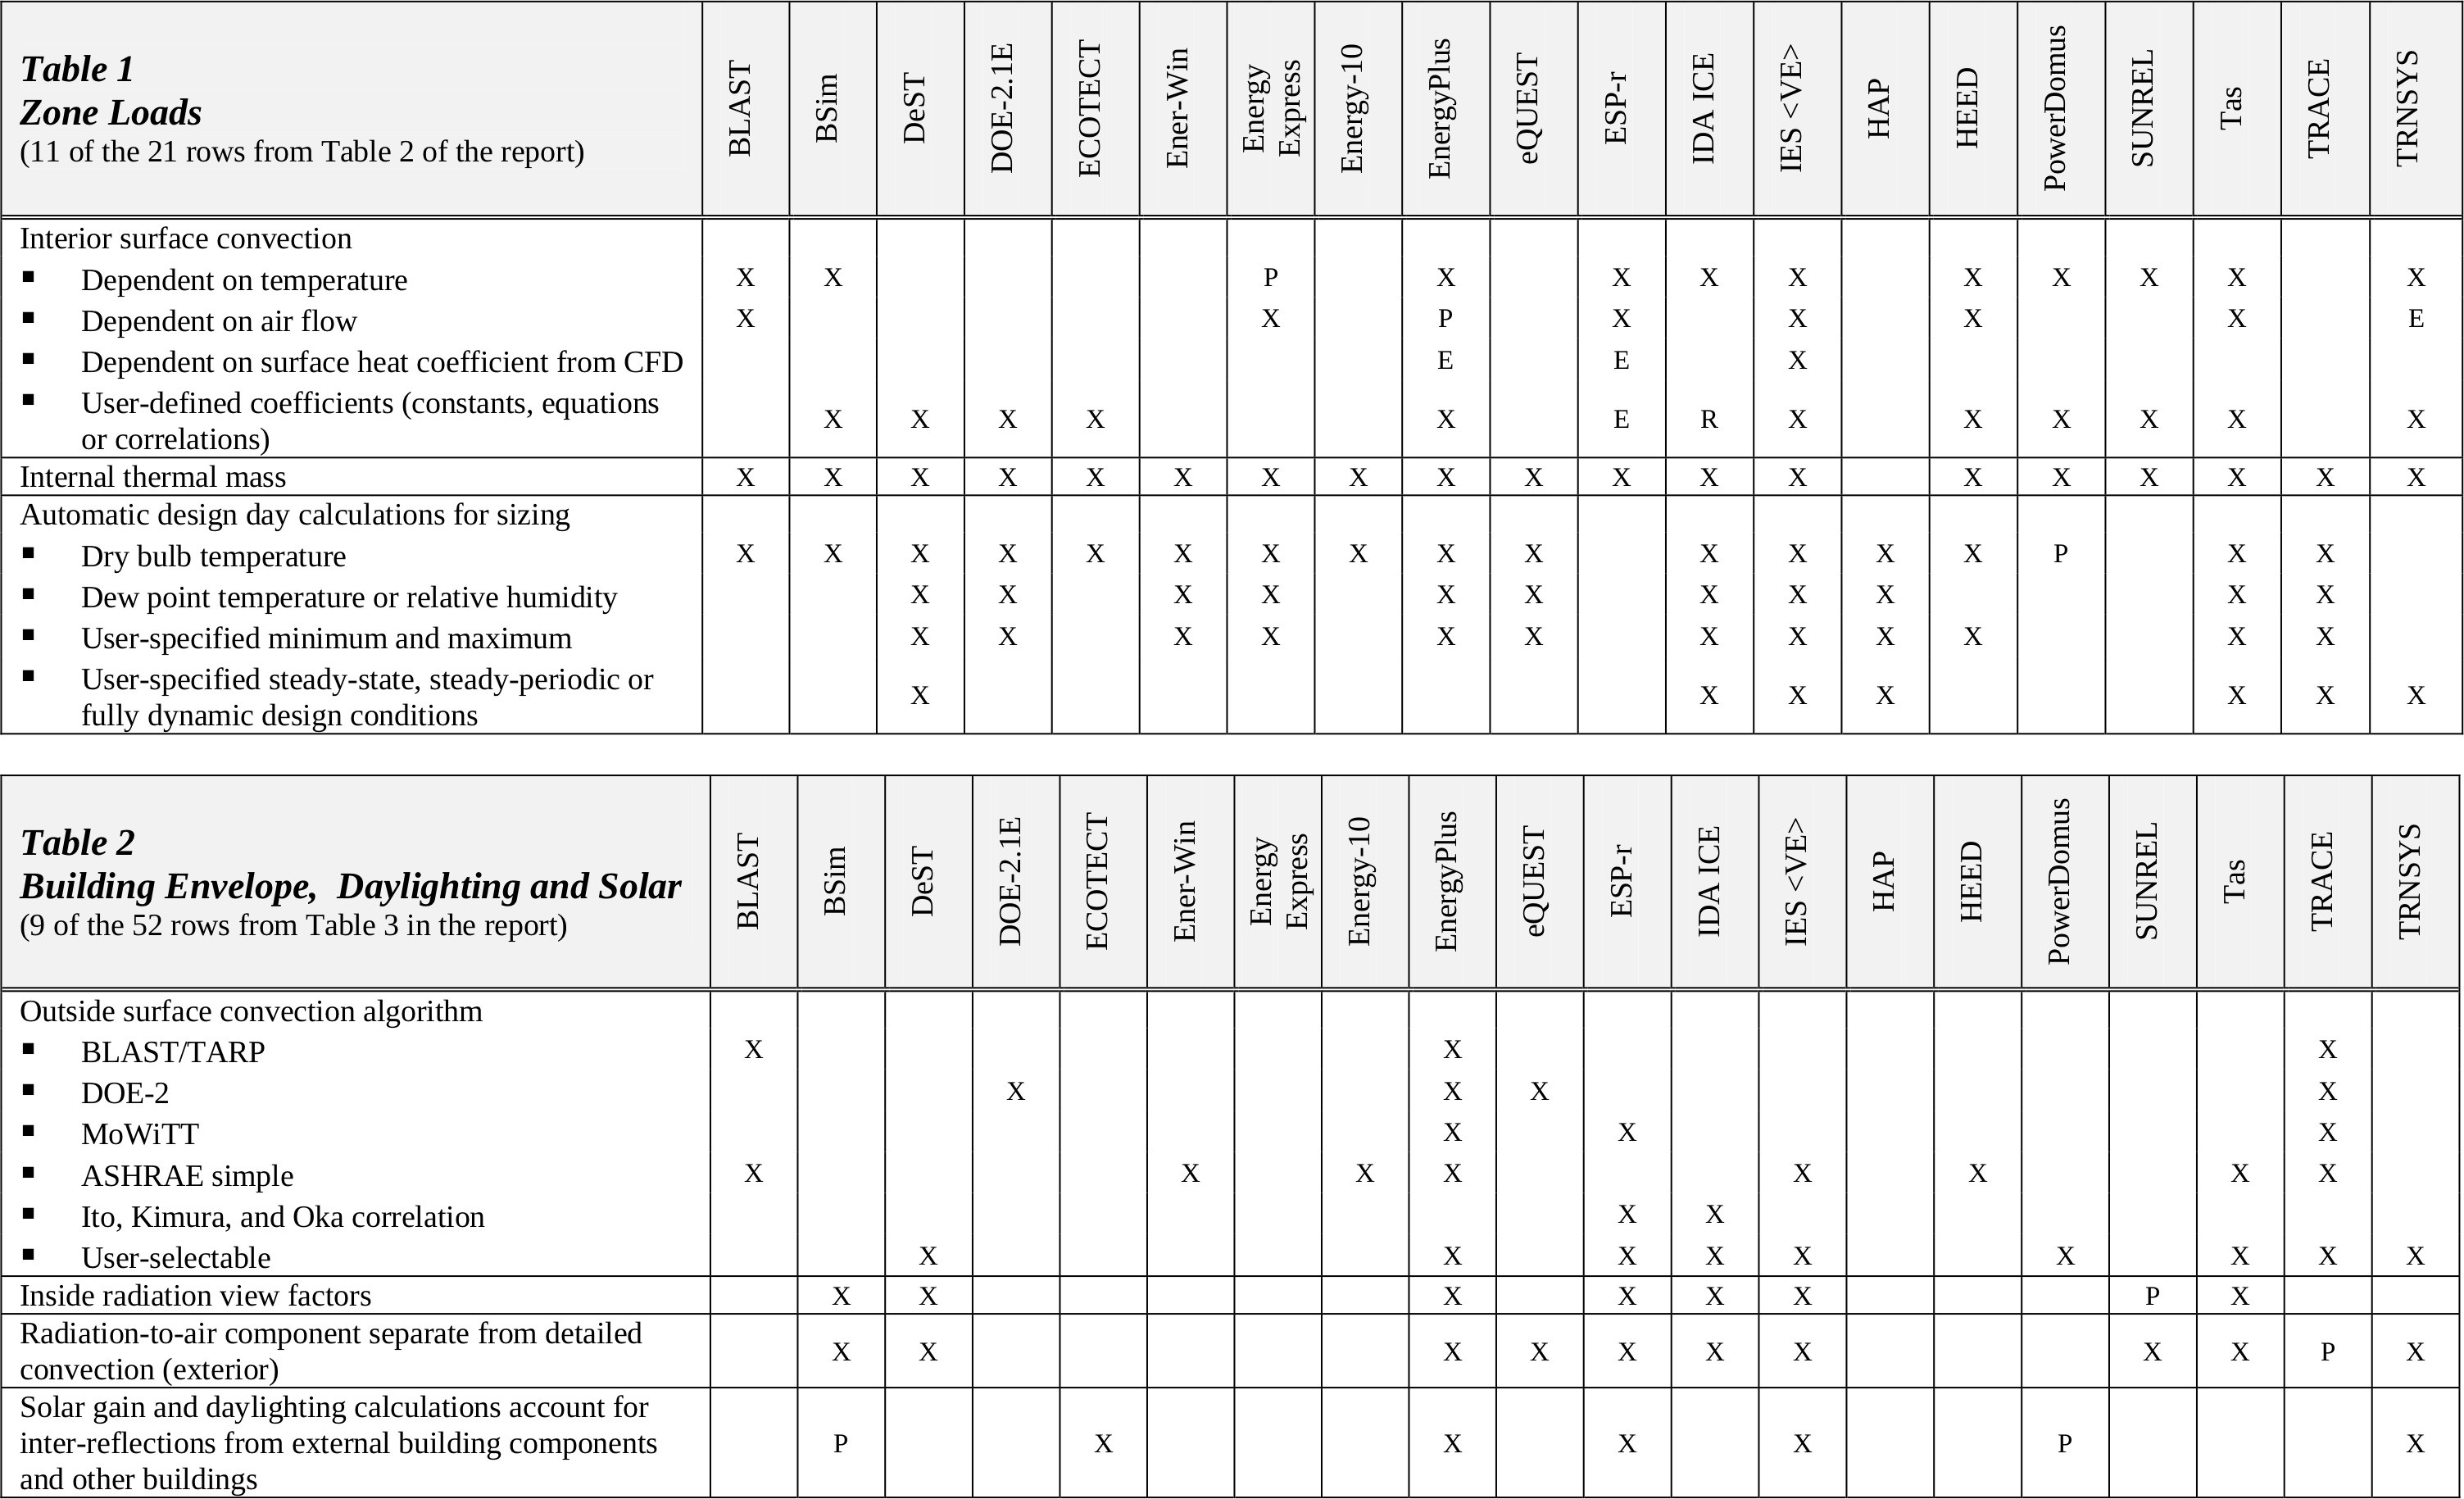
\includegraphics[width=\textwidth]{./Images/9-SimProg1}
\caption[Simulation Programs Comparative Analysis A]{A comparative analysis of programming schedules (Schedules 1, 2 and 3) \cite{crawley05}}
\label{fig:SimProg1}
\end{sidewaysfigure}

\begin{sidewaysfigure}[htbp]
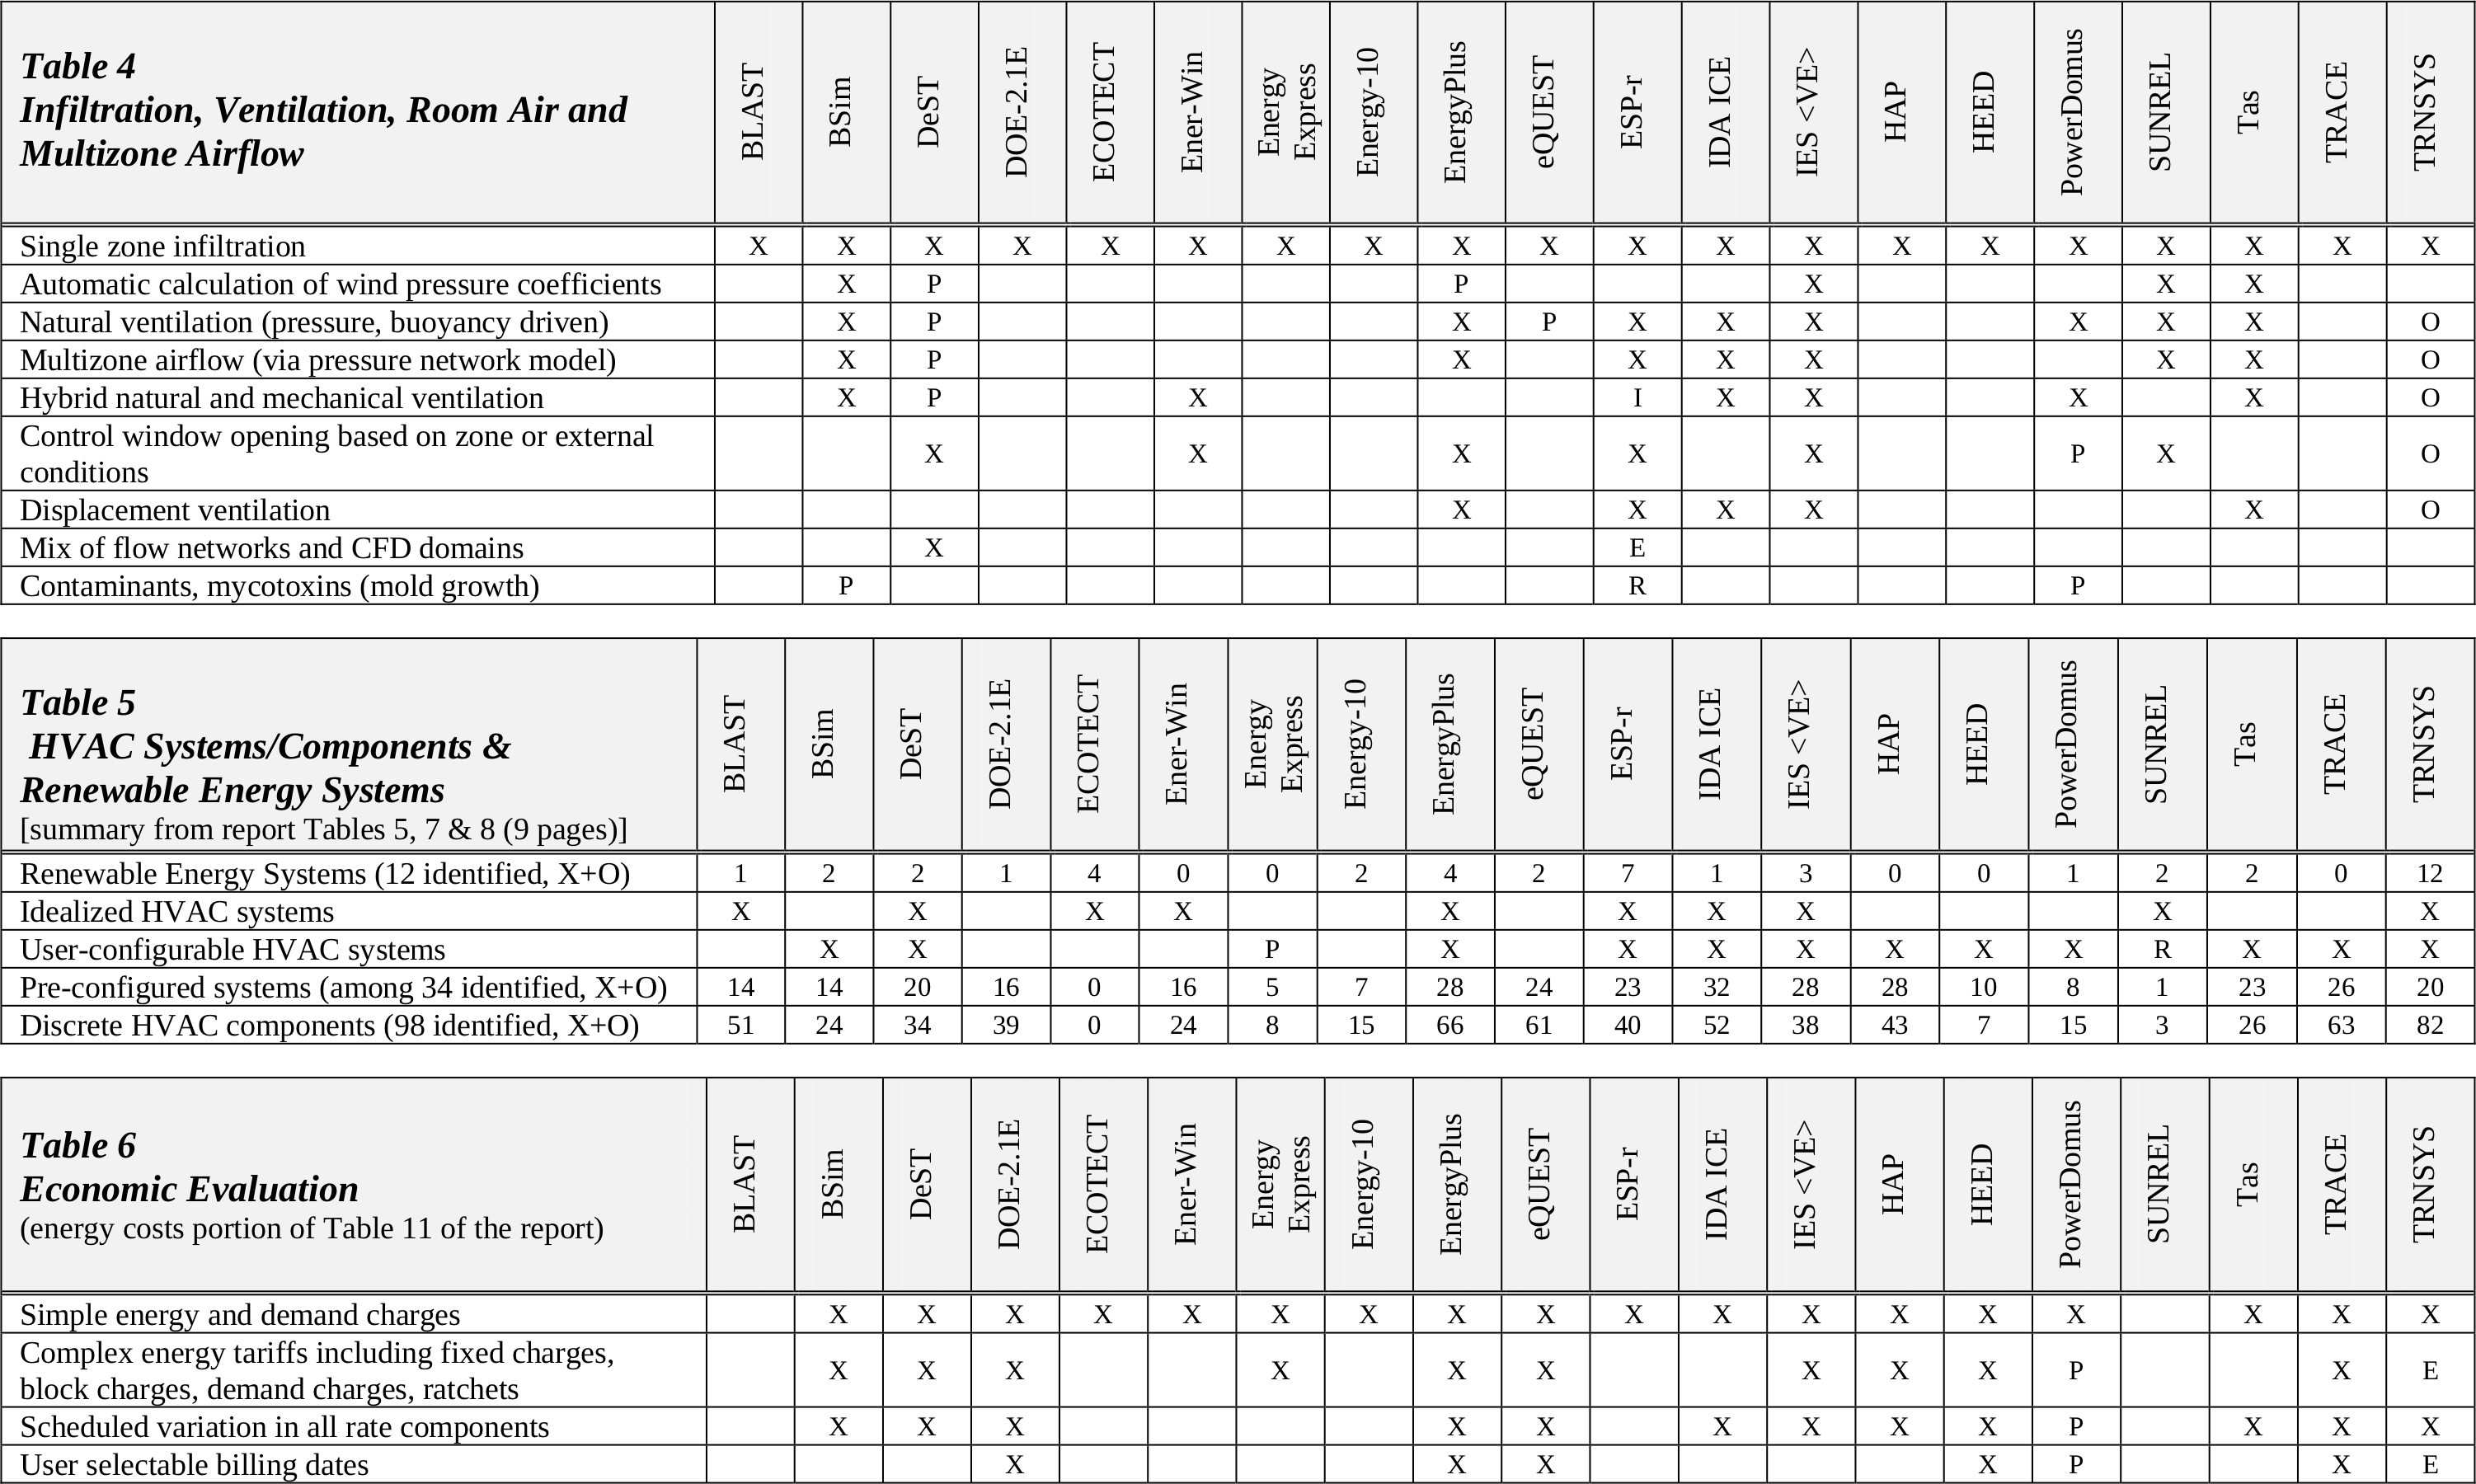
\includegraphics[width=\textwidth]{./Images/10-SimProg2}
\caption[Simulation Programs Comparative Analysis B]{A comparative analysis of programming schedules (Schedules 4, 5 and 6) \cite{crawley05}}
\label{fig:SimProg2}
\end{sidewaysfigure}
